% Chapter 5: VAR Models and Granger Causality
% Multivariate Time Series Analysis
% Bachelor program, Bucharest University of Economic Studies

\documentclass[9pt, aspectratio=169, t]{beamer}

% Ensure content fits on slides
\setbeamersize{text margin left=8mm, text margin right=8mm}

%=============================================================================
% THEME AND STYLE CONFIGURATION
%=============================================================================
\usetheme{Madrid}
\usecolortheme{seahorse}

% IDA-Inspired Color Palette
\definecolor{MainBlue}{RGB}{26, 58, 110}
\definecolor{AccentBlue}{RGB}{42, 82, 140}
\definecolor{IDAred}{RGB}{220, 53, 69}
\definecolor{DarkGray}{RGB}{51, 51, 51}
\definecolor{MediumGray}{RGB}{128, 128, 128}
\definecolor{LightGray}{RGB}{248, 248, 248}
\definecolor{VeryLightGray}{RGB}{235, 235, 235}
\definecolor{Crimson}{RGB}{220, 53, 69}
\definecolor{Forest}{RGB}{46, 125, 50}
\definecolor{Amber}{RGB}{181, 133, 63}
\definecolor{Orange}{RGB}{230, 126, 34}

\setbeamercolor{palette primary}{bg=MainBlue, fg=white}
\setbeamercolor{palette secondary}{bg=MainBlue!85, fg=white}
\setbeamercolor{palette tertiary}{bg=MainBlue!70, fg=white}
\setbeamercolor{structure}{fg=MainBlue}
\setbeamercolor{title}{fg=MainBlue}
\setbeamercolor{frametitle}{fg=MainBlue, bg=white}
\setbeamercolor{block title}{bg=MainBlue, fg=white}
\setbeamercolor{block body}{bg=VeryLightGray, fg=DarkGray}
\setbeamercolor{block title alerted}{bg=Crimson, fg=white}
\setbeamercolor{block body alerted}{bg=Crimson!8, fg=DarkGray}
\setbeamercolor{block title example}{bg=Forest, fg=white}
\setbeamercolor{block body example}{bg=Forest!8, fg=DarkGray}
\setbeamercolor{item}{fg=MainBlue}

\setbeamertemplate{navigation symbols}{}

\setbeamertemplate{footline}{
    \leavevmode%
    \hbox{%
        \begin{beamercolorbox}[wd=.333333\paperwidth,ht=2.5ex,dp=1ex,center]{author in head/foot}%
            \usebeamerfont{author in head/foot}\insertshortauthor
        \end{beamercolorbox}%
        \begin{beamercolorbox}[wd=.333333\paperwidth,ht=2.5ex,dp=1ex,center]{title in head/foot}%
            \usebeamerfont{title in head/foot}\insertshorttitle
        \end{beamercolorbox}%
        \begin{beamercolorbox}[wd=.333333\paperwidth,ht=2.5ex,dp=1ex,right]{date in head/foot}%
            \usebeamerfont{date in head/foot}\insertshortdate{}\hspace*{2em}
            \insertframenumber{} / \inserttotalframenumber\hspace*{2ex}
        \end{beamercolorbox}}%
    \vskip0pt%
}

%=============================================================================
% PACKAGES
%=============================================================================
\usepackage{amsmath, amssymb, amsthm}
\usepackage{mathtools}
\usepackage{bm}
\usepackage{tikz}
\usetikzlibrary{arrows.meta, positioning, shapes, calc}
\usepackage{booktabs}
\usepackage{multirow}
\usepackage{array}
\usepackage{graphicx}
\usepackage{hyperref}
\hypersetup{colorlinks=false, pdfborder={0 0 0}}
\graphicspath{{logos/}{charts/}}

%=============================================================================
% THEOREM ENVIRONMENTS
%=============================================================================
\theoremstyle{definition}
\setbeamertemplate{theorems}[numbered]
\newtheorem{defn}{Definition}
\newtheorem{thm}{Theorem}
\newtheorem{prop}{Proposition}

%=============================================================================
% CUSTOM COMMANDS
%=============================================================================
\newcommand{\E}{\mathbb{E}}
\newcommand{\Var}{\text{Var}}
\newcommand{\Cov}{\text{Cov}}
\newcommand{\Corr}{\text{Corr}}
\newcommand{\R}{\mathbb{R}}
\newcommand{\bY}{\mathbf{Y}}
\newcommand{\bX}{\mathbf{X}}
\newcommand{\bA}{\mathbf{A}}
\newcommand{\bB}{\mathbf{B}}
\newcommand{\bepsilon}{\boldsymbol{\varepsilon}}
\newcommand{\bSigma}{\boldsymbol{\Sigma}}

%=============================================================================
% TITLE INFORMATION
%=============================================================================
\title[Chapter 5: VAR \& Granger]{Chapter 5: VAR Models and Granger Causality}
\subtitle{Bachelor program Faculty of Cybernetics, Statistics and Economic Informatics, Bucharest University of Economic Studies, Romania}
\author[Prof. dr. Daniel Traian Pele]{Prof. dr. Daniel Traian Pele\\[0.2cm]\footnotesize\texttt{danpele@ase.ro}}
\institute{Bucharest University of Economic Studies}
\date{Academic Year 2025--2026}

\begin{document}

%=============================================================================
% TITLE SLIDE
%=============================================================================
\begin{frame}[plain]
    \begin{tikzpicture}[remember picture, overlay]
        \node[anchor=north west] at ([xshift=0.5cm, yshift=-0.3cm]current page.north west) {
            \href{https://www.ase.ro}{\includegraphics[height=1.1cm]{ase_logo.png}}
        };
        \node[anchor=north] at ([yshift=-0.3cm]current page.north) {
            \href{https://ai4efin.ase.ro}{\includegraphics[height=1.1cm]{ai4efin_logo.png}}
        };
        \node[anchor=north east] at ([xshift=-0.5cm, yshift=-0.3cm]current page.north east) {
            \href{https://www.digital-finance-msca.com}{\includegraphics[height=1.1cm]{msca_logo.png}}
        };
    \end{tikzpicture}
    \vfill
    \begin{center}
        {\Huge\textbf{\textcolor{MainBlue}{Chapter 5: VAR Models \& Granger Causality}}}\\[0.5cm]
        {\Large\textcolor{MainBlue}{Multivariate Time Series}}
    \end{center}
    \vfill

    \begin{tikzpicture}[remember picture, overlay]
        \node[anchor=south west] at ([xshift=0.5cm, yshift=0.8cm]current page.south west) {
            \href{https://theida.net}{\includegraphics[height=0.9cm]{ida_logo.png}}
        };
        \node[anchor=south] at ([xshift=-3cm, yshift=0.8cm]current page.south) {
            \href{https://blockchain-research-center.com}{\includegraphics[height=0.9cm]{brc_logo.png}}
        };
        \node[anchor=south] at ([yshift=0.8cm]current page.south) {
            \href{https://quantinar.com}{\includegraphics[height=0.9cm]{qr_logo.png}}
        };
        \node[anchor=south] at ([xshift=3cm, yshift=0.8cm]current page.south) {
            \href{https://quantlet.com}{\includegraphics[height=0.9cm]{ql_logo.png}}
        };
        \node[anchor=south east] at ([xshift=-0.5cm, yshift=0.8cm]current page.south east) {
            \href{https://ipe.ro/new}{\includegraphics[height=0.9cm]{acad_logo.png}}
        };
    \end{tikzpicture}
\end{frame}

%=============================================================================
% OUTLINE
%=============================================================================
\begin{frame}{Lecture Outline}
    \tableofcontents
\end{frame}

%=============================================================================
% SECTION 1: INTRODUCTION
%=============================================================================
\section{Introduction to Multivariate Time Series}

\begin{frame}{Why Multivariate Analysis?}
    \begin{block}{Limitations of Univariate Models}
        \begin{itemize}
            \item ARIMA models each variable \textbf{in isolation}
            \item Ignores potential \textbf{interactions} between variables
            \item Cannot capture \textbf{feedback effects}
        \end{itemize}
    \end{block}

    \vspace{0.15cm}

    \begin{exampleblock}{Economic Examples of Interdependence}
        \begin{itemize}
            \item GDP and unemployment (Okun's law)
            \item Interest rates and inflation (Taylor rule)
            \item Stock prices and trading volume
            \item Exchange rates and trade balance
        \end{itemize}
    \end{exampleblock}
\end{frame}

\begin{frame}{Multivariate Time Series Notation}
    \begin{block}{Vector of Variables}
        Let $\bY_t = (Y_{1t}, Y_{2t}, \ldots, Y_{Kt})'$ be a $K \times 1$ vector of time series.

        \vspace{0.2cm}
        Example with $K=2$:
        $$\bY_t = \begin{pmatrix} Y_{1t} \\ Y_{2t} \end{pmatrix} = \begin{pmatrix} \text{GDP growth}_t \\ \text{Inflation}_t \end{pmatrix}$$
    \end{block}

    \vspace{0.15cm}

    \begin{block}{Key Questions}
        \begin{enumerate}
            \item Does $Y_1$ help predict $Y_2$? (Granger causality)
            \item How do shocks to $Y_1$ affect $Y_2$? (Impulse responses)
            \item What proportion of $Y_2$'s variance is due to $Y_1$? (Variance decomposition)
        \end{enumerate}
    \end{block}
\end{frame}

%=============================================================================
% SECTION 2: VAR MODELS
%=============================================================================
\section{Vector Autoregression (VAR)}

\begin{frame}{The VAR(p) Model}
    \begin{block}{Definition}
        A \textbf{VAR(p)} model for $K$ variables:
        $$\bY_t = \mathbf{c} + \bA_1 \bY_{t-1} + \bA_2 \bY_{t-2} + \cdots + \bA_p \bY_{t-p} + \bepsilon_t$$

        where:
        \begin{itemize}
            \item $\bY_t$: $K \times 1$ vector of endogenous variables
            \item $\mathbf{c}$: $K \times 1$ vector of constants
            \item $\bA_i$: $K \times K$ coefficient matrices
            \item $\bepsilon_t$: $K \times 1$ vector of error terms with $\E[\bepsilon_t] = \mathbf{0}$, $\E[\bepsilon_t \bepsilon_t'] = \bSigma$
        \end{itemize}
    \end{block}
\end{frame}

\begin{frame}{VAR(1) with Two Variables}
    \begin{block}{Bivariate VAR(1)}
        $$\begin{pmatrix} Y_{1t} \\ Y_{2t} \end{pmatrix} = \begin{pmatrix} c_1 \\ c_2 \end{pmatrix} + \begin{pmatrix} a_{11} & a_{12} \\ a_{21} & a_{22} \end{pmatrix} \begin{pmatrix} Y_{1,t-1} \\ Y_{2,t-1} \end{pmatrix} + \begin{pmatrix} \varepsilon_{1t} \\ \varepsilon_{2t} \end{pmatrix}$$
    \end{block}

    \vspace{0.15cm}

    \begin{exampleblock}{Equation by Equation}
        \begin{align*}
            Y_{1t} &= c_1 + a_{11} Y_{1,t-1} + a_{12} Y_{2,t-1} + \varepsilon_{1t} \\
            Y_{2t} &= c_2 + a_{21} Y_{1,t-1} + a_{22} Y_{2,t-1} + \varepsilon_{2t}
        \end{align*}

        \textbf{Key insight}: Each equation includes lags of \textbf{all} variables!
    \end{exampleblock}
\end{frame}

\begin{frame}{Simulated VAR Process}
    \vspace{-0.3cm}
    \begin{center}
        \includegraphics[width=0.82\textwidth, height=0.58\textheight, keepaspectratio]{charts/ch5_var_simulation.pdf}
    \end{center}
    \vspace{-0.2cm}
    {\footnotesize
    \begin{itemize}
        \item Two simulated series from a bivariate VAR(1) process showing interdependence
        \item Each variable responds to both its own past and the other variable's past
        \item Notice how the series co-move due to cross-equation dynamics
    \end{itemize}
    }
\end{frame}

\begin{frame}{Stationarity of VAR}
    \begin{block}{Stability Condition}
        VAR(p) is \textbf{stable} (stationary) if all roots of:
        $$\det(\mathbf{I}_K - \bA_1 z - \bA_2 z^2 - \cdots - \bA_p z^p) = 0$$
        lie \textbf{outside} the unit circle (i.e., $|z| > 1$).
    \end{block}

    \vspace{0.15cm}

    \begin{alertblock}{For VAR(1)}
        The model is stable if all \textbf{eigenvalues} of $\bA_1$ are less than 1 in absolute value.

        \vspace{0.2cm}
        Example: For $\bA_1 = \begin{pmatrix} 0.5 & 0.1 \\ 0.2 & 0.3 \end{pmatrix}$, eigenvalues are $\lambda_1 = 0.6$ and $\lambda_2 = 0.2$.

        Both $< 1$ $\Rightarrow$ stable!
    \end{alertblock}
\end{frame}

\begin{frame}{Estimation of VAR}
    \begin{block}{OLS Estimation}
        Each equation can be estimated by \textbf{OLS separately}:
        $$\hat{\bA} = \left(\sum_{t=1}^{T} \bY_{t-1} \bY_{t-1}'\right)^{-1} \left(\sum_{t=1}^{T} \bY_{t-1} \bY_t'\right)$$

        \vspace{0.2cm}
        This is efficient because all equations have the \textbf{same regressors}.
    \end{block}

    \vspace{0.15cm}

    \begin{block}{Covariance Matrix}
        $$\hat{\bSigma} = \frac{1}{T-Kp-1} \sum_{t=1}^{T} \hat{\bepsilon}_t \hat{\bepsilon}_t'$$

        The errors $\varepsilon_{1t}$ and $\varepsilon_{2t}$ may be \textbf{contemporaneously correlated}.
    \end{block}
\end{frame}

\begin{frame}{Lag Order Selection}
    \begin{block}{Information Criteria}
        Choose $p$ that minimizes:
        \begin{align*}
            \text{AIC}(p) &= \ln|\hat{\bSigma}_p| + \frac{2pK^2}{T} \\[0.2cm]
            \text{BIC}(p) &= \ln|\hat{\bSigma}_p| + \frac{pK^2 \ln T}{T} \\[0.2cm]
            \text{HQ}(p) &= \ln|\hat{\bSigma}_p| + \frac{2pK^2 \ln\ln T}{T}
        \end{align*}
    \end{block}

    \vspace{0.2cm}

    {\small
    \begin{block}{Guidelines}
        \begin{itemize}
            \item AIC tends to select \textbf{larger} models (better for forecasting)
            \item BIC tends to select \textbf{smaller} models (consistent selection)
            \item Start with maximum $p_{max}$ based on data frequency (e.g., 4 for quarterly, 12 for monthly)
        \end{itemize}
    \end{block}
    }
\end{frame}

%=============================================================================
% SECTION 3: GRANGER CAUSALITY
%=============================================================================
\section{Granger Causality}

\begin{frame}{What is Granger Causality?}
    \begin{block}{Clive Granger (1969, Nobel Prize 2003)}
        ``$X$ \textbf{Granger-causes} $Y$'' if past values of $X$ help predict $Y$, \textbf{beyond} what past values of $Y$ alone can predict.
    \end{block}

    \vspace{0.15cm}

    \begin{alertblock}{Important Distinction}
        \textbf{Granger causality $\neq$ True causality}

        \begin{itemize}
            \item Granger causality is about \textbf{predictive content}
            \item Does NOT imply economic/structural causation
            \item ``$X$ Granger-causes $Y$'' means: $X$ contains useful information for forecasting $Y$
        \end{itemize}
    \end{alertblock}
\end{frame}

\begin{frame}{Formal Definition}
    \begin{block}{Granger Causality}
        $X$ \textbf{does not Granger-cause} $Y$ if:
        $$\E[Y_t | Y_{t-1}, Y_{t-2}, \ldots, X_{t-1}, X_{t-2}, \ldots] = \E[Y_t | Y_{t-1}, Y_{t-2}, \ldots]$$

        In other words: adding $X$'s history does not improve the prediction of $Y$.
    \end{block}

    \vspace{0.15cm}

    \begin{exampleblock}{In the VAR Context}
        For VAR(1): $Y_{1t} = c_1 + a_{11} Y_{1,t-1} + a_{12} Y_{2,t-1} + \varepsilon_{1t}$

        \vspace{0.2cm}
        $Y_2$ does \textbf{not} Granger-cause $Y_1$ if $a_{12} = 0$.

        \vspace{0.2cm}
        For VAR(p): $Y_2$ does not Granger-cause $Y_1$ if $a_{12}^{(1)} = a_{12}^{(2)} = \cdots = a_{12}^{(p)} = 0$.
    \end{exampleblock}
\end{frame}

\begin{frame}{Testing for Granger Causality}
    \begin{block}{Hypothesis Test}
        \textbf{$H_0$}: $Y_2$ does \textbf{not} Granger-cause $Y_1$

        $$H_0: a_{12}^{(1)} = a_{12}^{(2)} = \cdots = a_{12}^{(p)} = 0$$

        \textbf{$H_1$}: At least one $a_{12}^{(i)} \neq 0$ (Granger causality exists)
    \end{block}

    \vspace{0.15cm}

    \begin{block}{Test Statistic: Wald Test}
        $$F = \frac{(RSS_R - RSS_U)/p}{RSS_U/(T-2p-1)} \sim F_{p, T-2p-1}$$

        where:
        \begin{itemize}
            \item $RSS_R$: Residual sum of squares from restricted model (without $Y_2$ lags)
            \item $RSS_U$: Residual sum of squares from unrestricted model (full VAR)
        \end{itemize}
    \end{block}
\end{frame}

\begin{frame}{Types of Granger Causality}
    \begin{center}
    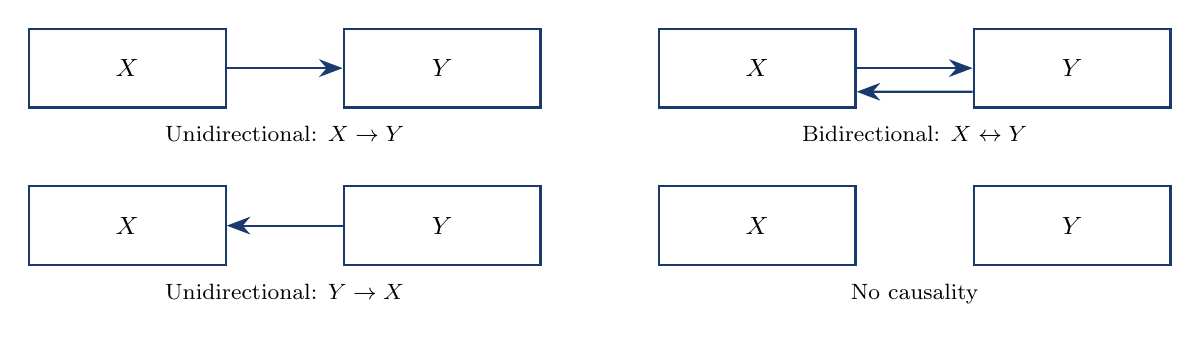
\begin{tikzpicture}[
        box/.style={rectangle, draw=MainBlue, thick, minimum width=2.5cm, minimum height=1cm, font=\small},
        arrow/.style={-{Stealth[length=3mm]}, thick, MainBlue}
    ]
        % Unidirectional X -> Y
        \node[box] (x1) at (0, 2) {$X$};
        \node[box] (y1) at (4, 2) {$Y$};
        \draw[arrow] (x1) -- (y1);
        \node[below=0.1cm of x1, xshift=2cm, font=\footnotesize] {Unidirectional: $X \rightarrow Y$};

        % Unidirectional Y -> X
        \node[box] (x2) at (0, 0) {$X$};
        \node[box] (y2) at (4, 0) {$Y$};
        \draw[arrow] (y2) -- (x2);
        \node[below=0.1cm of x2, xshift=2cm, font=\footnotesize] {Unidirectional: $Y \rightarrow X$};

        % Bidirectional
        \node[box] (x3) at (8, 2) {$X$};
        \node[box] (y3) at (12, 2) {$Y$};
        \draw[arrow] (x3.east) -- (y3.west);
        \draw[arrow] (y3.west) ++(0, -0.3) -- (x3.east |- {0, 1.7});
        \node[below=0.1cm of x3, xshift=2cm, font=\footnotesize] {Bidirectional: $X \leftrightarrow Y$};

        % No causality
        \node[box] (x4) at (8, 0) {$X$};
        \node[box] (y4) at (12, 0) {$Y$};
        \node[below=0.1cm of x4, xshift=2cm, font=\footnotesize] {No causality};
    \end{tikzpicture}
    \end{center}

    \vspace{0.15cm}

    {\small
    \begin{block}{Economic Examples}
        \begin{itemize}
            \item Money $\rightarrow$ Output? (monetarist view)
            \item Stock prices $\leftrightarrow$ Trading volume (bidirectional)
            \item Weather $\rightarrow$ Crop yields (unidirectional, obvious)
        \end{itemize}
    \end{block}
    }
\end{frame}

\begin{frame}{Cross-Correlation Function}
    {\small
    \begin{defn}[Cross-Correlation Function]
        The \textbf{cross-correlation} between $X_t$ and $Y_t$ at lag $k$ is:
        $$\rho_{XY}(k) = \frac{\gamma_{XY}(k)}{\sigma_X \sigma_Y} = \frac{\Cov(X_t, Y_{t+k})}{\sqrt{\Var(X_t)\Var(Y_t)}}$$
    \end{defn}

    \begin{block}{Interpretation}
        \begin{itemize}\setlength{\itemsep}{0pt}
            \item $\rho_{XY}(k) > 0$ at $k > 0$: $X$ is positively correlated with future $Y$ (X may lead Y)
            \item $\rho_{XY}(k) > 0$ at $k < 0$: $X$ is positively correlated with past $Y$ (Y may lead X)
        \end{itemize}
    \end{block}

    \begin{alertblock}{Note}
        Unlike ACF, cross-correlation is \textbf{not symmetric}: $\rho_{XY}(k) \neq \rho_{XY}(-k)$ in general.
    \end{alertblock}
    }
\end{frame}

\begin{frame}{Cross-Correlation Analysis}
    \vspace{-0.3cm}
    \begin{center}
        \includegraphics[width=0.82\textwidth, height=0.58\textheight, keepaspectratio]{charts/ch5_cross_correlation.pdf}
    \end{center}
    \vspace{-0.2cm}
    {\footnotesize
    \begin{itemize}
        \item Cross-correlation function measures linear dependence at different lags
        \item Significant correlations at negative lags suggest $X$ leads $Y$; positive lags suggest $Y$ leads $X$
        \item Useful for preliminary analysis before formal Granger causality testing
    \end{itemize}
    }
\end{frame}

\begin{frame}{Granger Causality: Practical Considerations}
    \begin{alertblock}{Common Pitfalls}
        \begin{enumerate}
            \item \textbf{Omitted variables}: A third variable $Z$ may cause both $X$ and $Y$
            \item \textbf{Non-stationarity}: Test requires stationary data (or cointegration)
            \item \textbf{Lag selection}: Results can be sensitive to $p$
            \item \textbf{Sample size}: Need sufficient observations
        \end{enumerate}
    \end{alertblock}

    \vspace{0.15cm}

    \begin{block}{Best Practices}
        \begin{itemize}
            \item Test for unit roots first
            \item Use multiple lag selection criteria
            \item Check robustness to different lag lengths
            \item Report results for both directions
        \end{itemize}
    \end{block}
\end{frame}

%=============================================================================
% SECTION 4: IMPULSE RESPONSE FUNCTIONS
%=============================================================================
\section{Impulse Response Functions}

\begin{frame}{What are Impulse Response Functions?}
    \begin{block}{Definition}
        An \textbf{Impulse Response Function (IRF)} traces the effect of a one-time shock to one variable on the current and future values of all variables.
    \end{block}

    \vspace{0.15cm}

    \begin{exampleblock}{Question IRFs Answer}
        ``If there is an unexpected 1-unit shock to $Y_1$ today, what happens to $Y_1$ and $Y_2$ over the next $h$ periods?''
    \end{exampleblock}

    \vspace{0.15cm}

    \begin{block}{MA($\infty$) Representation}
        A stable VAR(p) can be written as:
        $$\bY_t = \boldsymbol{\mu} + \sum_{i=0}^{\infty} \boldsymbol{\Phi}_i \bepsilon_{t-i}$$

        The matrices $\boldsymbol{\Phi}_i$ are the \textbf{impulse responses} at horizon $i$.
    \end{block}
\end{frame}

\begin{frame}{Computing IRFs for VAR(1)}
    \begin{block}{For VAR(1): $\bY_t = \mathbf{c} + \bA \bY_{t-1} + \bepsilon_t$}
        The impulse response matrices are:
        $$\boldsymbol{\Phi}_0 = \mathbf{I}_K, \quad \boldsymbol{\Phi}_1 = \bA, \quad \boldsymbol{\Phi}_2 = \bA^2, \quad \ldots, \quad \boldsymbol{\Phi}_h = \bA^h$$
    \end{block}

    \vspace{0.15cm}

    \begin{exampleblock}{Interpretation}
        $[\boldsymbol{\Phi}_h]_{ij}$ = Effect on $Y_i$ at time $t+h$ of a unit shock to $Y_j$ at time $t$

        \vspace{0.2cm}
        For stable VAR: $\boldsymbol{\Phi}_h \rightarrow \mathbf{0}$ as $h \rightarrow \infty$ (shocks die out)
    \end{exampleblock}
\end{frame}

\begin{frame}{Computing IRFs for General VAR(p)}
    {\small
    \begin{block}{Recursive Formula for VAR(p)}
        For $\bY_t = \mathbf{c} + \bA_1\bY_{t-1} + \bA_2\bY_{t-2} + \cdots + \bA_p\bY_{t-p} + \bepsilon_t$:
        $$\boldsymbol{\Phi}_h = \sum_{j=1}^{\min(h,p)} \bA_j \boldsymbol{\Phi}_{h-j}, \quad h = 1, 2, 3, \ldots$$
        with $\boldsymbol{\Phi}_0 = \mathbf{I}_K$ and $\boldsymbol{\Phi}_h = \mathbf{0}$ for $h < 0$.
    \end{block}

    \begin{exampleblock}{Example: VAR(2) IRFs}
        \begin{itemize}\setlength{\itemsep}{0pt}
            \item $\boldsymbol{\Phi}_0 = \mathbf{I}_K$
            \item $\boldsymbol{\Phi}_1 = \bA_1 \boldsymbol{\Phi}_0 = \bA_1$
            \item $\boldsymbol{\Phi}_2 = \bA_1 \boldsymbol{\Phi}_1 + \bA_2 \boldsymbol{\Phi}_0 = \bA_1^2 + \bA_2$
            \item $\boldsymbol{\Phi}_3 = \bA_1 \boldsymbol{\Phi}_2 + \bA_2 \boldsymbol{\Phi}_1 = \bA_1(\bA_1^2 + \bA_2) + \bA_2\bA_1$
        \end{itemize}
    \end{exampleblock}
    }
\end{frame}

\begin{frame}{Orthogonalized IRFs}
    \begin{alertblock}{Problem: Correlated Errors}
        If $\bSigma$ is not diagonal, shocks $\varepsilon_{1t}$ and $\varepsilon_{2t}$ are correlated.

        A shock to ``$Y_1$'' also involves a shock to ``$Y_2$''.
    \end{alertblock}

    \vspace{0.15cm}

    \begin{block}{Solution: Cholesky Decomposition}
        Factor $\bSigma = \mathbf{P}\mathbf{P}'$ where $\mathbf{P}$ is lower triangular.

        Define orthogonalized shocks: $\mathbf{u}_t = \mathbf{P}^{-1}\bepsilon_t$ with $\E[\mathbf{u}_t \mathbf{u}_t'] = \mathbf{I}$

        \vspace{0.2cm}
        Orthogonalized IRFs: $\boldsymbol{\Theta}_h = \boldsymbol{\Phi}_h \mathbf{P}$
    \end{block}

    \vspace{0.2cm}

    {\small
    \begin{alertblock}{Ordering Matters!}
        Cholesky assumes variables ordered from ``most exogenous'' to ``most endogenous''. Results depend on this ordering.
    \end{alertblock}
    }
\end{frame}

\begin{frame}{Impulse Response Functions: Example}
    \vspace{-0.3cm}
    \begin{center}
        \includegraphics[width=0.82\textwidth, height=0.58\textheight, keepaspectratio]{charts/ch5_irf.pdf}
    \end{center}
    \vspace{-0.2cm}
    {\footnotesize
    \begin{itemize}
        \item IRFs show how each variable responds to a one-unit shock over time
        \item Shaded regions represent confidence intervals (uncertainty in estimates)
        \item For stable VAR models, responses converge to zero as the horizon increases
    \end{itemize}
    }
\end{frame}

%=============================================================================
% SECTION 5: FORECAST ERROR VARIANCE DECOMPOSITION
%=============================================================================
\section{Forecast Error Variance Decomposition}

\begin{frame}{Variance Decomposition}
    \begin{block}{Question}
        What proportion of the forecast error variance of $Y_i$ at horizon $h$ is due to shocks to $Y_j$?
    \end{block}

    \vspace{0.15cm}

    \begin{block}{FEVD Formula}
        $$\text{FEVD}_{ij}(h) = \frac{\sum_{s=0}^{h-1} [\boldsymbol{\Theta}_s]_{ij}^2}{\sum_{s=0}^{h-1} \sum_{k=1}^{K} [\boldsymbol{\Theta}_s]_{ik}^2}$$

        \vspace{0.2cm}
        This gives the \textbf{percentage} of $Y_i$'s $h$-step forecast variance explained by shocks to $Y_j$.
    \end{block}

    \vspace{0.2cm}

    {\small
    \begin{exampleblock}{Properties}
        \begin{itemize}
            \item $0 \leq \text{FEVD}_{ij}(h) \leq 1$
            \item $\sum_{j=1}^{K} \text{FEVD}_{ij}(h) = 1$ (sums to 100\%)
            \item At $h=1$: Own shocks dominate (by construction with Cholesky)
        \end{itemize}
    \end{exampleblock}
    }
\end{frame}

\begin{frame}{FEVD: Example}
    \vspace{-0.3cm}
    \begin{center}
        \includegraphics[width=0.82\textwidth, height=0.58\textheight, keepaspectratio]{charts/ch5_fevd.pdf}
    \end{center}
    \vspace{-0.2cm}
    {\footnotesize
    \begin{itemize}
        \item FEVD shows the proportion of forecast variance attributable to each shock
        \item At short horizons, own shocks dominate; cross-variable effects grow over time
        \item Useful for understanding the relative importance of different shocks in the system
    \end{itemize}
    }
\end{frame}

%=============================================================================
% SECTION 6: PRACTICAL EXAMPLE
%=============================================================================
\section{Practical Example}

\begin{frame}{Example: GDP and Unemployment}
    \begin{block}{Okun's Law}
        There is a negative relationship between GDP growth and unemployment:
        $$\Delta U_t \approx -\beta (\Delta Y_t - \bar{g})$$

        where $\bar{g}$ is trend GDP growth and $\beta \approx 0.4$.
    \end{block}

    \vspace{0.15cm}

    \begin{exampleblock}{VAR Analysis Questions}
        \begin{enumerate}
            \item Does GDP growth Granger-cause unemployment changes?
            \item Does unemployment Granger-cause GDP growth?
            \item How do shocks propagate between variables?
        \end{enumerate}
    \end{exampleblock}
\end{frame}

\begin{frame}{GDP and Unemployment: Data}
    \vspace{-0.3cm}
    \begin{center}
        \includegraphics[width=0.82\textwidth, height=0.58\textheight, keepaspectratio]{charts/ch5_gdp_unemployment.pdf}
    \end{center}
    \vspace{-0.2cm}
    {\footnotesize
    \begin{itemize}
        \item GDP growth and unemployment rate show clear negative correlation (Okun's Law)
        \item Both series exhibit cyclical patterns related to business cycle fluctuations
        \item This bivariate system is ideal for VAR analysis and Granger causality testing
    \end{itemize}
    }
\end{frame}

\begin{frame}{VAR Workflow}
    \begin{enumerate}
        \item \textbf{Data preparation}
            \begin{itemize}
                \item Check for stationarity (unit root tests)
                \item Transform if necessary (differences, logs)
            \end{itemize}

        \vspace{0.2cm}
        \item \textbf{Lag selection}
            \begin{itemize}
                \item Use AIC, BIC, HQ criteria
                \item Check residual autocorrelation
            \end{itemize}

        \vspace{0.2cm}
        \item \textbf{Estimation}
            \begin{itemize}
                \item OLS equation by equation
                \item Check stability (eigenvalues)
            \end{itemize}

        \vspace{0.2cm}
        \item \textbf{Analysis}
            \begin{itemize}
                \item Granger causality tests
                \item Impulse response functions
                \item Variance decomposition
            \end{itemize}

        \vspace{0.2cm}
        \item \textbf{Forecasting}
    \end{enumerate}
\end{frame}

\begin{frame}[fragile]{Python Implementation}
    \begin{block}{VAR in Python (statsmodels)}
        \footnotesize
\begin{verbatim}
from statsmodels.tsa.api import VAR
from statsmodels.tsa.stattools import grangercausalitytests

# Fit VAR model
model = VAR(data)
results = model.fit(maxlags=4, ic='aic')

# Granger causality test
granger_test = grangercausalitytests(data[['Y1', 'Y2']],
                                      maxlag=4)
# Impulse response functions
irf = results.irf(periods=20)
irf.plot()

# Variance decomposition
fevd = results.fevd(periods=20)
fevd.plot()
\end{verbatim}
    \end{block}
\end{frame}

%=============================================================================
% SECTION 7: SUMMARY
%=============================================================================
\section{Summary}

\begin{frame}{Key Takeaways}
    {\footnotesize
    \begin{block}{VAR Models}
        \begin{itemize}\setlength{\itemsep}{0pt}
            \item Model \textbf{multiple} time series jointly
            \item Each variable depends on its own lags AND lags of other variables
            \item Estimated by OLS equation by equation; requires stationarity
        \end{itemize}
    \end{block}

    \begin{block}{Granger Causality}
        \begin{itemize}\setlength{\itemsep}{0pt}
            \item Tests whether $X$ helps predict $Y$ beyond $Y$'s own history
            \item \textbf{Not} the same as true causality; F-test on coefficient restrictions
        \end{itemize}
    \end{block}

    \begin{block}{IRF and FEVD}
        \begin{itemize}\setlength{\itemsep}{0pt}
            \item IRF: How shocks propagate through the system
            \item FEVD: What proportion of variance is due to each shock
            \item Both depend on variable ordering (Cholesky decomposition)
        \end{itemize}
    \end{block}
    }
\end{frame}

\begin{frame}{What's Next?}
    \begin{alertblock}{Topics for Further Study}
        \begin{itemize}
            \item \textbf{Cointegration}: Long-run relationships between non-stationary variables
            \item \textbf{VECM}: Error correction models for cointegrated systems
            \item \textbf{Structural VAR}: Imposing economic theory restrictions
            \item \textbf{Panel VAR}: VAR for panel data
        \end{itemize}
    \end{alertblock}

    \vspace{0.25cm}

    \begin{center}
        \Large\textcolor{MainBlue}{Questions?}
    \end{center}
\end{frame}

\end{document}
